
The probabilities from the data set are in the following output excerpt:
Probabilities for Each Class:
% \begin{center}    
%     \captionof{Probabilities for Each Class\label{tab:probabilities}}
%     \begin{tabular}{cc}
%         \hline
%         Class & Probability \\
%         \hline
%         3.0 & 0.5007 \\
%         4.0 & 0.2503 \\
%         9.0 & 0.1251 \\
%         6.0 & 0.0626 \\
%         2.0 & 0.0313 \\
%         0.0 & 0.0156 \\
%         5.0 & 0.0078 \\
%         8.0 & 0.0038 \\
%         1.0 & 0.0019 \\
%         7.0 & 0.0009 \\
%         \hline
%     \end{tabular}    
% \end{center}
%If we inspect the histogram of the incoming true classes we see the results in figure~\ref{fig:histogram}. 
%However, the results of the classification are shown in figure~\ref{fig:classification}.

\begin{center}    
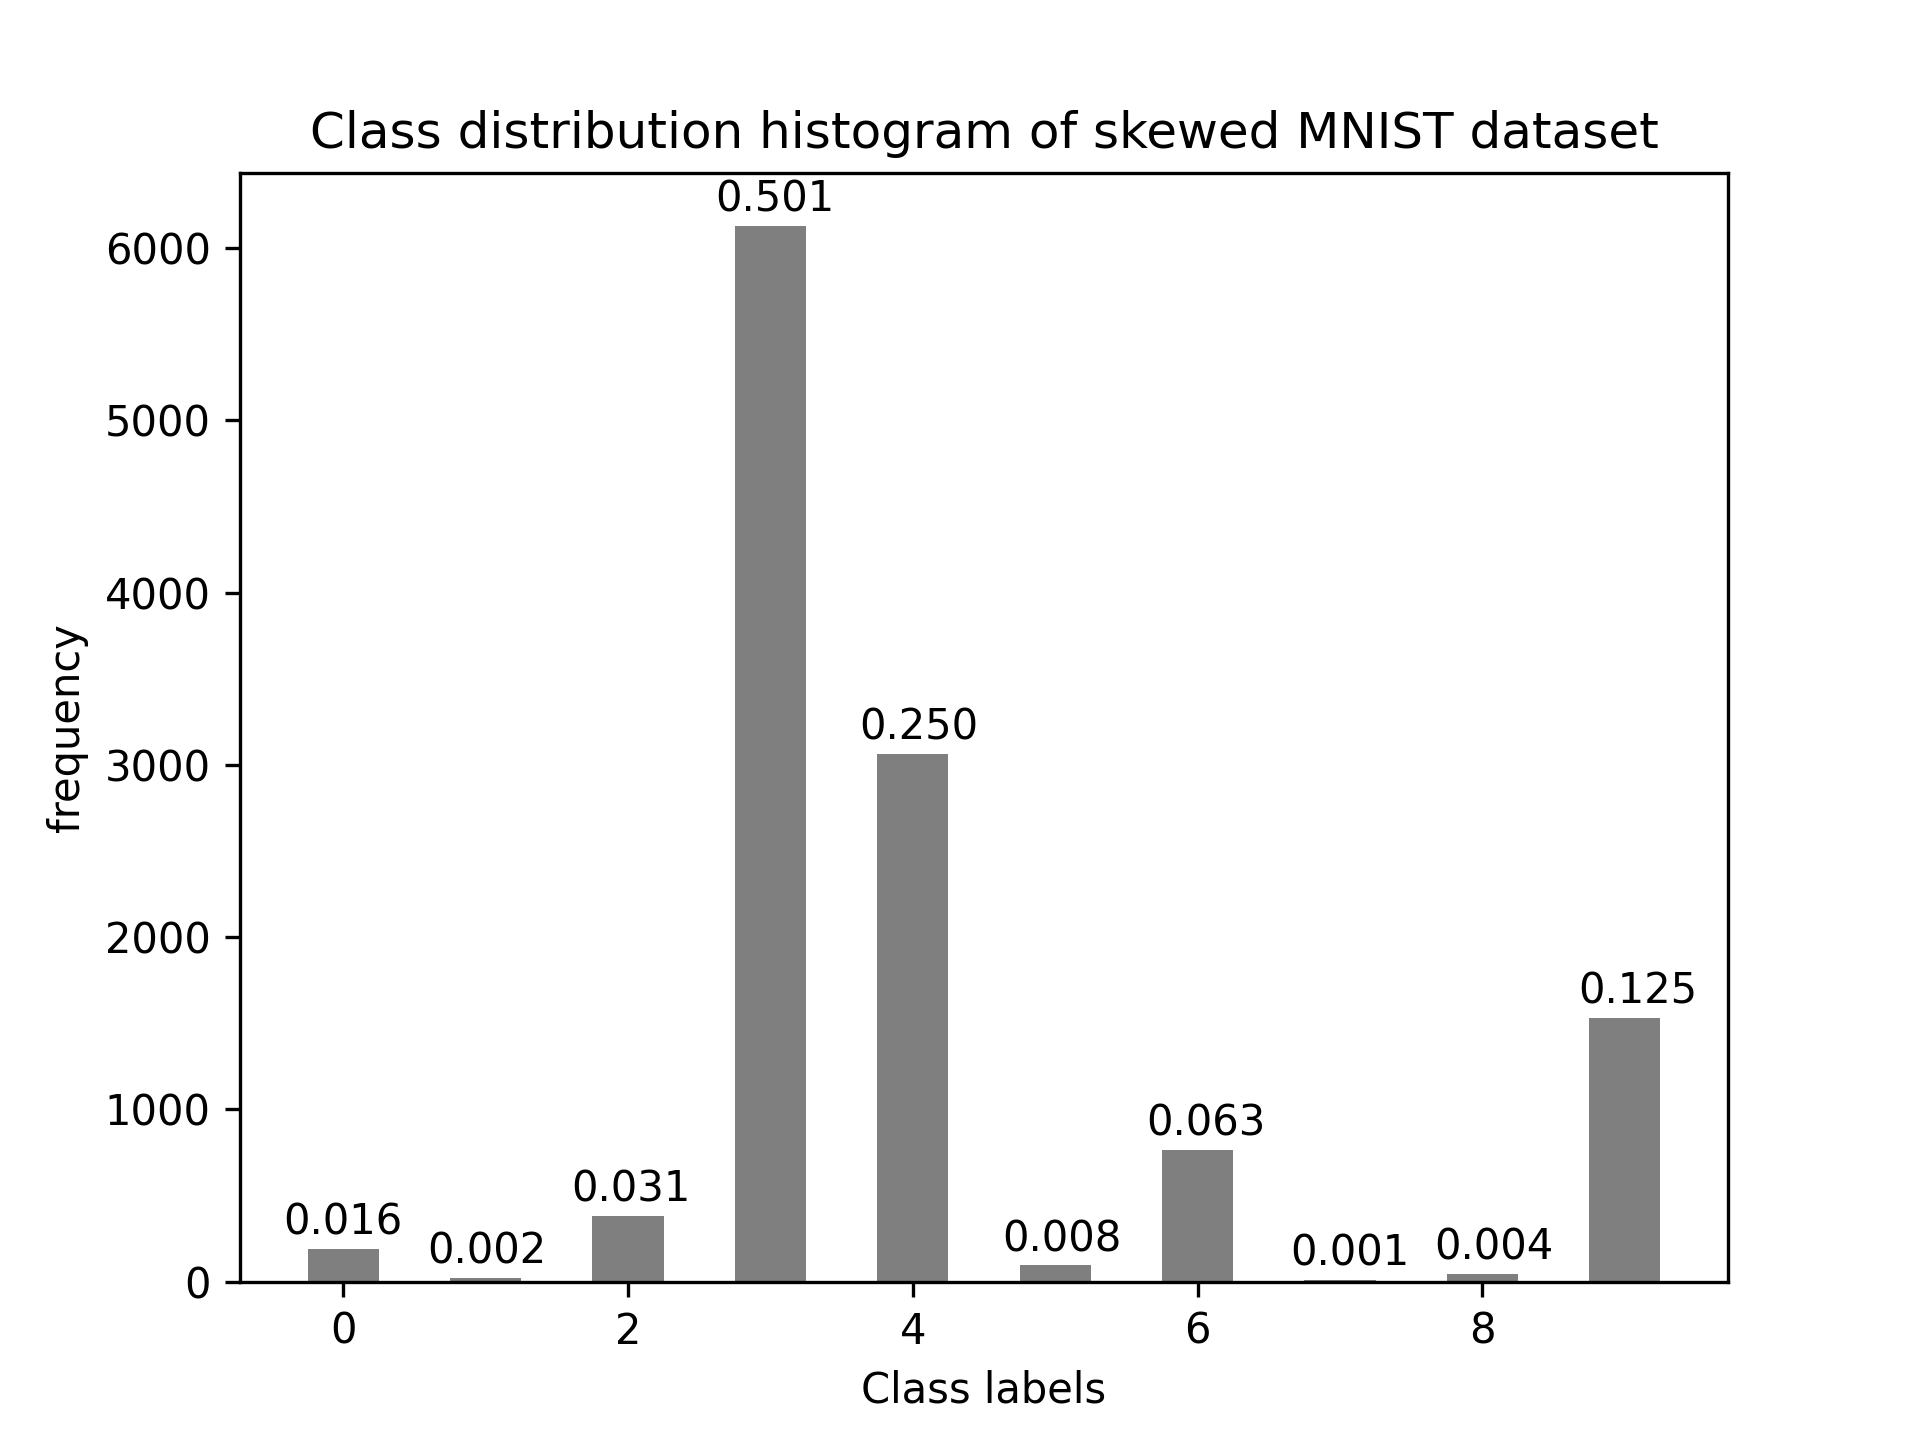
\includegraphics[width=0.5\textwidth]{class_histogram.png}
%\captionof{Histogram of True Classes\label{fig:histogram}}
\end{center}    


\begin{center}    
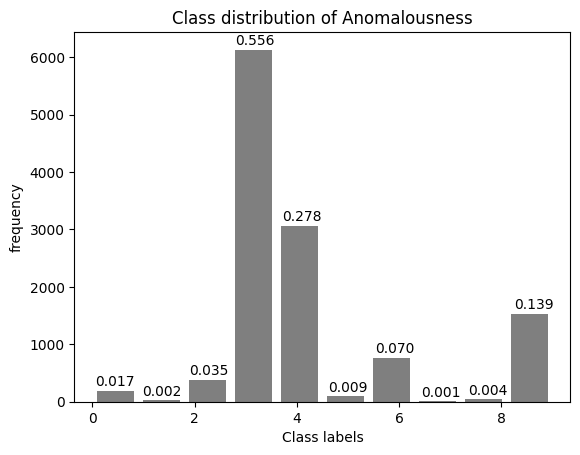
\includegraphics[width=0.5\textwidth]{class_histogram_anomalousness.png}
%\captionof{Histogram of Classification Results\label{fig:classification}}    
\end{center}
The accuracy of the method was 0.65485, or 65.5~\%.

